\section{Numerical Experiments}
\label{sec:experiments}
Two baselines are defined for the numerical experiments, which are referred to as $\text{Baseline}_\text{0A}$ and $\text{Baseline}_\text{0B}$. In each experiment, one or more parameters are varied, while the rest are left as in either one of these baselines. The parameter values were selected through a trial and error procedure with the following goals:
\acomment{cosa significa questa cosa?}
\begin{itemize}
	\item
	$\#$ of people sufficiently large in order not too have a too large variance over different experiments with same parameters.
	\item
	Reasonable computation time per experiment.
	\item
	Reasonable average number of connections per individual.
	\item
	Chi più ne ha, più ne metta
\end{itemize}
Table \ref{table:1} summarizes the parameter values of $\text{Baseline}_\text{0A}$. \newline
The parameter values of $\text{Baseline}_\text{0B}$ are the same as in $\text{Baseline}_\text{0A}$ but for the probability distribution of the traits, which are illustrated in Table \ref{table:2}.
\begin{table}[h!]
\centering
\begin{tabular}{||c | c || c | c ||}
	\hline
	Parameter&Value&Parameter&Value\\
	\hline
	$C$&0.2&Range& $\begin{bmatrix} 0.1n_{People} \\ 0.1 n_{People}\end{bmatrix}$\\
	$n_{Root}$&4&Locality&$\begin{bmatrix} True \\ True\end{bmatrix}$\\
	$n_{People}$&100&Similarity&$\delta(x-0.5)$\\
	$n_{Fake}$&2&Crit. Thinking&$\delta(x-0.5)$\\
	$n_{Real}$&2&Influenceability&$\delta(x-0.5)$\\
	\hline
\end{tabular}
\newline
\caption{$\text{Baseline}_\text{0A}$ parameter values. When a bidimensional vector is given, the first component refers to the real news sources and the second component refers to the fake news sources. $\delta(x)$ is a vector for the entire population, where each component is a delta-dirac function.}
\label{table:1}
\end{table}
\begin{table}[h!]
\centering
	\begin{tabular}{||c | c||}
	\hline
	Parameter&Value\\
	\hline
	Similarity&$U(0,1)$\\
	Crit. Thinking&$U(0,1)$\\
	Influenceability&$U(0,1)$\\
	\hline
	\end{tabular}
	\newline
	\caption{$\text{Baseline}_\text{0B}$ personality distributions of the propulation.}
	\label{table:2}
\end{table}
\subsection{Instruction Level}
\label{sec:Instr_Level}
The goal of the numerical experiments presented in this section is investigating the effect of the \emph{instruction level} on the population's steady state opinions. The instruction level $\in [0,1]$ models the capacity of people to identify whether a source is spreading real or fake news. It therefore affects the trait \emph{critical thinking}. A function $f$ is defined that maps an instruction level to its corresponding critical thinking probability distribution:
$$
f: [0,1] \to p 
$$
$$
p:= \{g,\ g: [0,1] \to \mathbb{R}_+,\ \int_{0}^{1} g(x) \,dx = 1\}
$$
In order to obtain this mapping, the beta distribution is employed: 
$$
f(\text{level}) = Beta(\alpha(\text{level}), \beta(\text{level}))\text{, level} \in [0,1]
$$
$$
P(CT_i\in[x,x+dx]) = [f(\text{level})](x)\times dx\text{, x}\in [0,1]
$$
, where $CT_i$ is the critical thinking parameter for individual i. The relationships between the instruction level and $\alpha$ and $\beta$ are provided in the code in the appendix. 
\begin{figure}[!t]
	\centering
	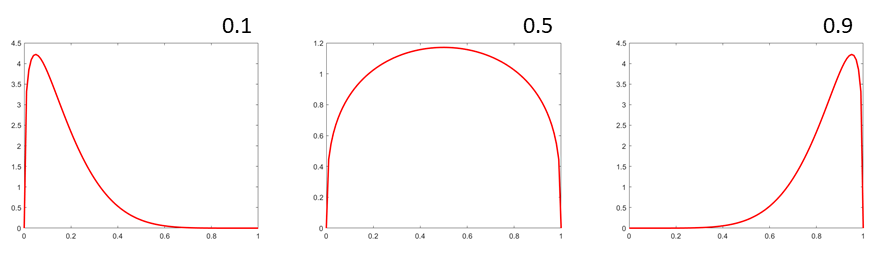
\includegraphics[width=3.5in]{Figures/instruction_level_dist.png}
	\caption{Critical thinking probability distribution for instruction level = \{0.1, 0.5, 0.9\}.}
	\label{pics:critdistribution}
\end{figure}
Figure~\ref{pics:critdistribution} shows the critical thinking probability distribution for three examples of instruction level. A higher instruction level implies a more critical society with the distribution peak moving to the right (= higher critical thinking coefficient). Vice versa, a low instruction level moves the distribution peak to the left (lower critical thinking coefficient). \newline
\begin{figure}[!t]
	\centering
	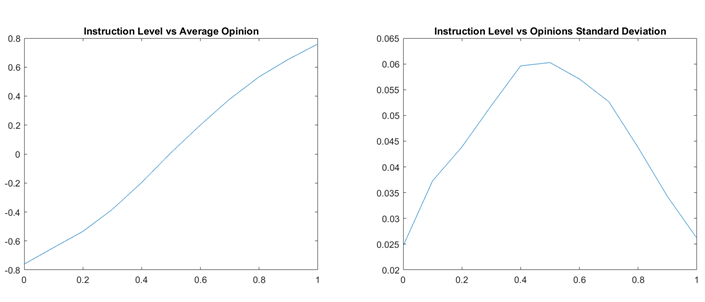
\includegraphics[width=3.5in]{Figures/instruction_results.png}
	\caption{Average Opinion and Opinions Standard Deviation for instruction level = 0:0.1:1}
	\label{pics:critstatistics}
\end{figure}
In the experiments, the parameter instruction level is varied in its whole range [0,1] and the average opinion and the opinions standard deviation are computed. The rest of the parameters are left as in $\text{Baseline}_\text{0B}$. For each instruction level, 100 cases have been randomly generated and the average metrics have been computed for the steady state opinions.
Figure~\ref{pics:critstatistics} shows the results. As expected, the higher the instruction level the closer the average opinion to 1 and vice versa the lower the instruction level, the closer the average opinion to -1. Furthermore, as the peak gets sharper (either on the right or on the left side) the standard deviation decreases. The opinion therefore converges to values close to 1 (or -1) and the standard deviation decreases as $|level-0.5|$ increases. 
\subsection{Society Diversity}
The goal of the numerical experiment presented in this section is investigating the effect of the diversity factor $\alpha$ on the transient and steady state behavior of the network opinions. The parameter $\alpha \in \mathbb{R}$ models the diversity in the network. It therefore affects the trait $similarity$.
A function f maps a value of $\alpha$ to its corresponding similarity probability distribution. 
$$
f: \mathbb{R} \to p 
$$
$$
p:= \{g,\ g: \mathbb{R} \to \mathbb{R}_+,\ \int_{-\infty}^{\infty} g(x) \,dx = 1\}
$$
In order to obtain this mapping, a simple uniform distribution is employed:
$$
f(\alpha) = U(-\alpha, \alpha), \alpha \in \mathbb{R}
$$
$$
P(S_i\in[x,x+dx]) =  \frac{1}{2\alpha} \times dx\text{, x}\in [-\alpha, \alpha]
$$
where $S_i$ is the similarity coefficient of individual i.
The diversity in the society increases as $\alpha$ increases. Each possible similarity value occurs with the same probability but as $\alpha$ increases, the spectrum of possibilities gets larger. \newline
In the experiments, the parameter $\alpha$ is varied in [0,50] and the average opinion and the opinions standard deviation are computed. Furthermore the length of the transient phase is recorded. The rest of the parameters are left as in $\text{Baseline}_\text{0B}$. For each $\alpha$, 100 cases have been randomly generated and the average metrics have been computed for the steady state opinions. 

\begin{figure}[!t]
	\centering
	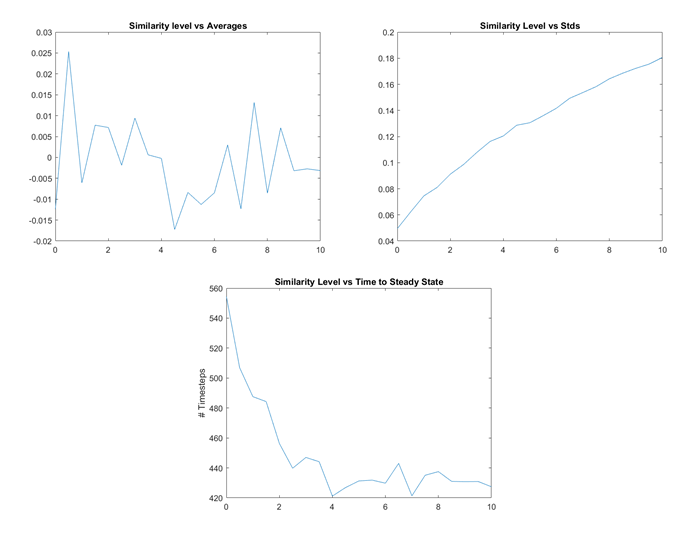
\includegraphics[width=3.5in]{Figures/diversity_results.png}
	\caption{Average Opinion, Opinions Standard Deviation and time to steady state for $\alpha$ = 0:1:50.}
	\label{pics:diversityresults}
\end{figure}
Figure~\ref{pics:diversityresults} illustrates the results. The average opinion does not show any trend as it oscillates around the value zero. This is expected since no opinion is preferred with this set up. By contrast, the standard deviation increases with $\alpha$. In a more diverse society, there is a larger variety of groups sharing the same view of things. People belonging to a group will prefer to stick to that group opinion. The steady state will therefore show a greater variety of opinions with the resulting larger standard deviation. Finally, the parameter time to steady state shows an initial decrease from $\approx$ 550 to $\approx$ 430 timesteps for $\alpha \in [0,10]$ and then it starts increasing with an approximately linear trend for the rest of the time. 

\subsection{Population manipulability}
In this experiment, the goal is to investigate how modifying the \textit{Influenceability} parameter of the population affects the time to convergence of the opinions in the population. Qualitatively, this would be equivalent to study how well ideas spread in a "stubborn" population versus a highly manipulable population. If one thinks about the real world, the speed of idea spreading is a very important concept. A society with very stubborn individuals may be more stable, and on the other hand change is propelled by people with a flexible view on new ideas. \acomment{magari citare qualcosa, o mettere questo trafiletto in un altro posto}
We define the manipulability level $\in [0,1]$ of the society and study how this affects the time to convergence of the opinion dynamics. A manipulability level of $0$ represents a society difficult to manipulate, while a manipulability level of $1$ represents a society where people are more influenceable. Again, this is modelled through the beta distribution, in a similar fashion as in Subsection~\ref{sec:Instr_Level}. This time, however, the \textit{influenceability} is modelled trhough the beta distribution. For the numerical experiments, the manipulability level is varied in the range $[0,1]$ and the other parameters are left as in $\text{Baseline}_\text{0B}$. The experiment is repeated 100 times and the results are averaged. A plot showing that the average time to steady state decreases when the society is more manipulable can be found in Figure~\ref{pics:man_steadystate}. In the range of manipualibility level $[0,1]$, the time to steady state goes from around a maximum of $\approx 580$ timesteps to a minimum of $\approx 480$ timesteps. The result is in line with expectations: the less influenceable individuals are, and the larger weights of the self-loops in the graph will be. For individuals, this corresponds to favoring their own ideas instead of the neighbors' ones and "slowing" thus the information propagation in the network.
\begin{figure}[!t]
	\centering
	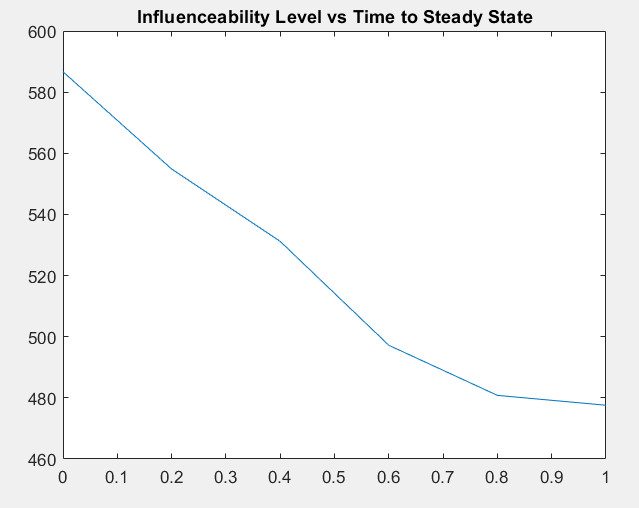
\includegraphics[width=3.5in]{Figures/Exp8_2.png}
	\caption{Average timesteps necessary to reach steady state with varying the manipulability level in the range $[0,1]$.}
\label{pics:man_steadystate}
\end{figure}


\subsection{Polarization}

The goal of the numerical experiments presented in this section is investigating the opinion polarization within a population using our model. In particular, we aim to understand how the model parameters influence the polarization. 
Polarization refers either to a distribution of opinions with multiple local maxima or to the process by which such strong divergences of opinions that divide a population come about \cite{Banisch2019}\cite{Bramsona2016}. The model presented in Section~\ref{sec:mathematical} has been slightly modified for what concerns the link weights. If $s_i$ denotes the similarity of individual $i$, then the entry $a_{ij} = a_{ji}$ is 
\begin{equation}
a_{ij} = \text{max}\{0, \delta_{ij} + 0.2\ r\}
\end{equation}
where $r$ is a random number from normal distribution $\mathcal{N}(0,1)$ and $\delta_{ij} = 1$ if $s_i = s_j$ otherwise $\delta_{ij} = 0$. 

The number of real and fake sources is 3. Influencability and critical thinking traits are set to $0.5$ for all individuals. Similarity is set to $1$ for half of individuals and to $0$ for the second half. Thus, the probability of creating a link remains the same, but the weight of the link has is around 1 if the node belong to the same half and non-negative and close to 0 if they belong to different halves. An example of a single experiment is shown in Figure~\ref{pics:exp20}.\\

\begin{figure}[!t]
\centering
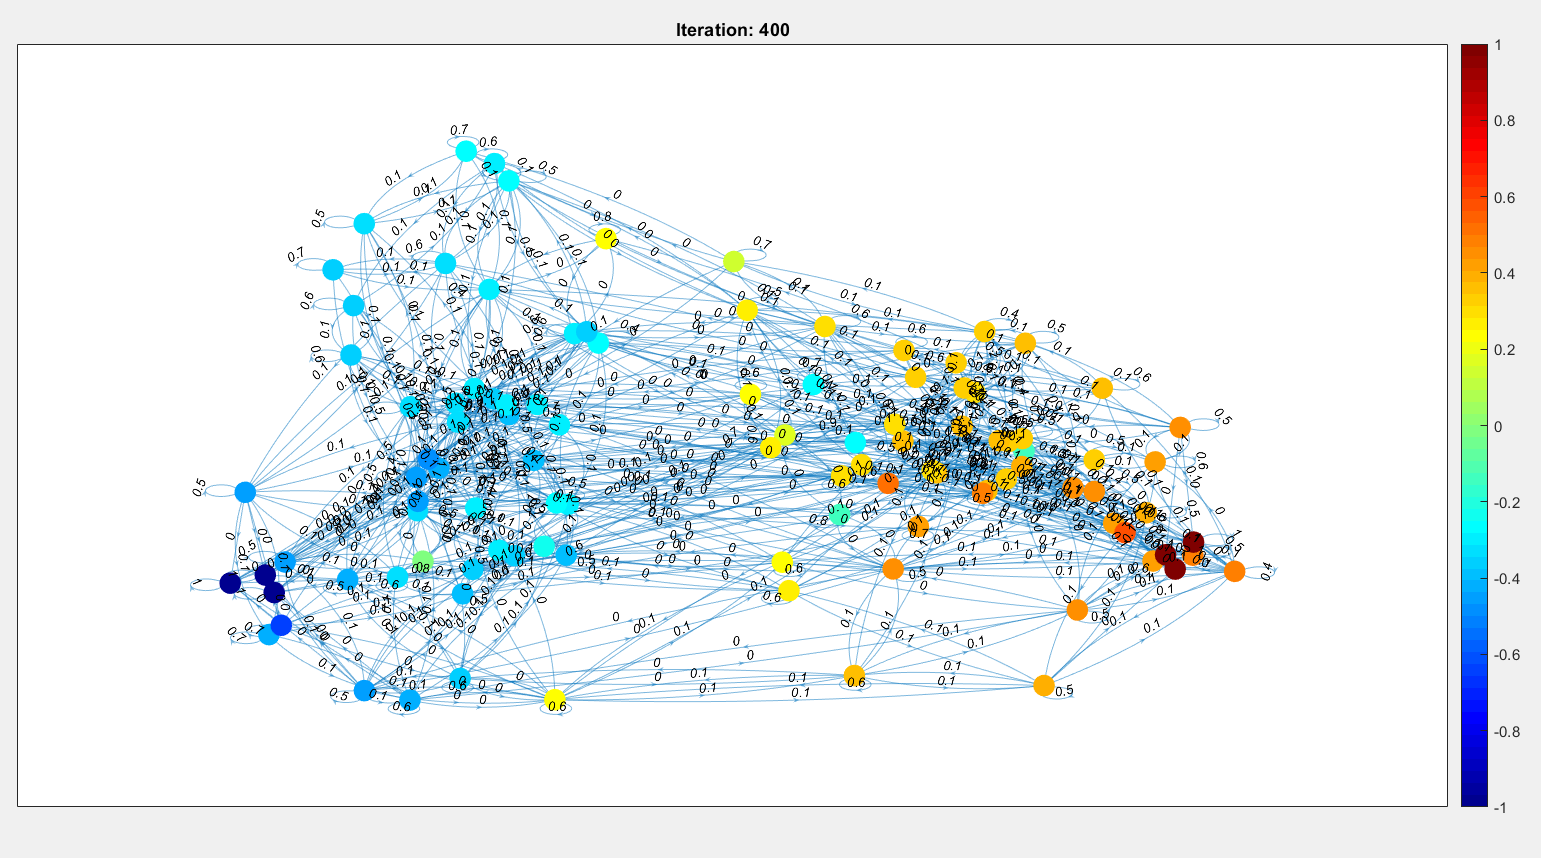
\includegraphics[width=8cm]{Figures/Exp20_graph.png}
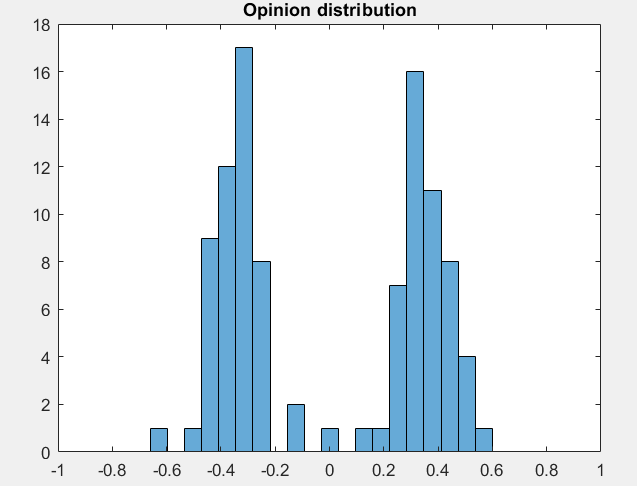
\includegraphics[width=8cm]{Figures/Exp20_hyst.png}
\caption{Simulation with 100 individuals, 3 sources of Fake and 3 of Real News, $C=0.2$, nRoot$=4$ and new connection local. Above: graph at steady state. Below: opinion distribution at steady sate.}
\label{pics:exp20}
\end{figure}

To the best of our knowledge, there is not a unique metric to quantify opinion polarization. We used the measure proposed in \cite{Matakos2017} defined as $R_2 = ||x_{\infty}||^2/ N$, the standard deviation of $x_{\infty}$ according to the interpretation of polarization as dispersion exposed in \cite{Bramsona2016} and the mean.\\

In our experiments, we varied three parameters: $C$ in the range $[0.2; 0.6]$, nRoot in the range $[2; 8]$ and the news connection, which is either local or spread. For each parameters combination, 100 cases have been randomly generated and the average metrics have been computed for the opinion vector at steady state.\\

The mean is at  $0 \pm 5\times 10^{-3}$ for all cases, which means that there is not a predominant opinion. This is expected, because the parametrization does not favour one opinion. When the news sources are spread, the average is even closer to 0 ($0 \pm 10^{-3}$). Although in this section we are not interested in the average opinion, the fact that the mean is close to 0 makes the standard deviation and $R_2$ good metrics to evaluate the polarization. A high standard deviation correspond to many entries far from the center on both sides of the opinion spectrum.\\

Because of the mean $\overline{x}$ close to 0 and $N=100$, we have
$$ \sigma^2 = \frac{1}{N-1} \sum_{i=1}^N (x_i-\overline{x})^2 \approx \frac{1}{N} \sum_{i=1}^N x_i^2 = R_2.$$

Thus, the two metrics carry the same information about the polarization and, for sake of simplicity, we only discuss the standard deviation. Results for 30 parameters combinations are shown in Figure~\ref{pics:pol_std}. Since the opinions are between $-1$ and $1$, the standard deviation is between 0 and 1.\\

We notice that the higher $C$ and nRoot are, the less polarized are the opinions. Moreover, the higher lower nRoot is, the faster grows the polarization by decreasing $C$. This is in line with our expectations. The higher is $C$, the more likely contacts are and is proportional to the average in and out degree of each node. A high nRoot means that each individual is more likely to have a link with another individual which is far and, in this case, contacts among individuals with different similarity are more likely. Thus, the experiments show that polarization arises in the society when individuals are in contact with few other people or when they are in contact mainly with similar people. The strongest polarization is present when both conditions are met.\\

Another remarkable result is the comparison between the cases where the news are local (blue) and when they are spread (red). Spreading the news reduces the polarization in the network. 
For each $C$ and nRoot combination, the standard deviation is at most one third of the value for the corresponding case with local news. Also with spread news we observe an increase of polarization when $C$ and nRoot decrease, but the growth is less strong. This experiment suggest that a society where each individual has the chance to come in touch with all news sources and not only the ones close to their milieu, is less likely be polarized.
\acomment{riferimento a letteratura? evitare di dare troppo significato!}
\acomment{numerazione pagine manca}
\acomment{descrizione di esperimento Social diversity poco chiara}
\acomment{dire chiaramente nella teoria che A (la parte tra individui è simmetrica?}
%\begin{algorithm}
%\While {i > 0}{Do this}
%\end{algorithm}
\begin{figure}[!t]
\centering
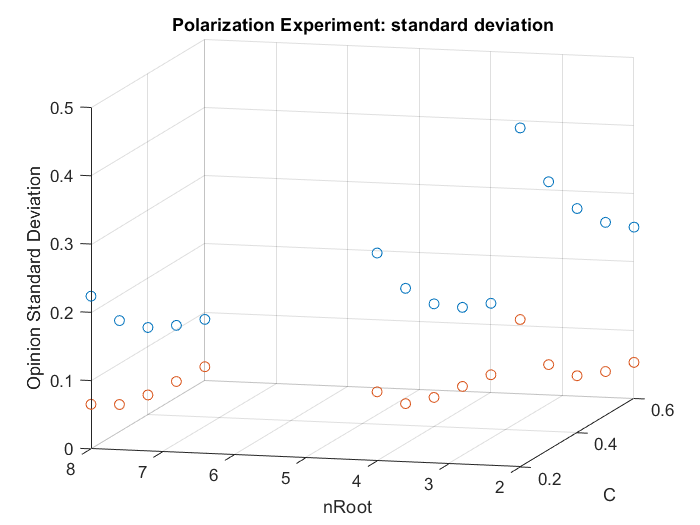
\includegraphics[width=8cm]{Figures/pol_std1.png}
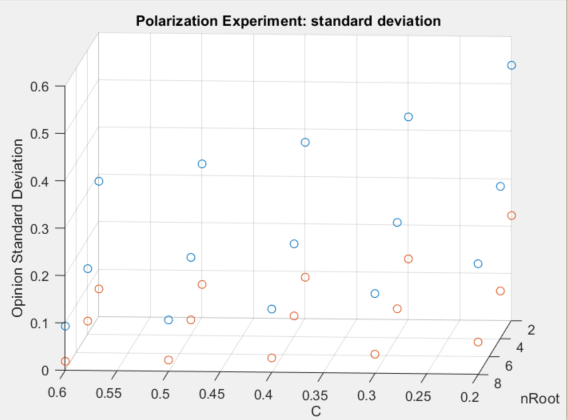
\includegraphics[width=8cm]{Figures/pol_std2.png}
\caption{Standard deviation for different combinations of C, nRoot and news connection. Red: news are spread. Blue: news are local.}
\label{pics:pol_std}
\end{figure}










